\documentclass[10pt,a4paper]{article}
\usepackage[utf8]{inputenc}
\usepackage{amsmath}
\usepackage{bm}
\usepackage{amsfonts}
\usepackage{amssymb}
\usepackage{tikz}
\usepackage[left=2cm,right=2cm,top=2cm,bottom=2cm]{geometry}
\usepackage{graphicx}
\usepackage{subcaption}


\usepackage{algorithm}
\usepackage[noend]{algpseudocode}
\makeatletter
\def\BState{\State\hskip-\ALG@thistlm}
\makeatother


\begin{document}

\title{Averaged Control}
\author{Víctor Hernández-Santamaría \thanks{DeustoTech, University of Deusto.} \and José Vicente Lorenzo Gómez \thanks{Universidad Autónoma de Madrid.} \and Enrique Zuazua ${}^*$}

\maketitle

In this work, we address the optimal control of parameter-dependent systems. We introduce the notion of averaged control in which the quantity of interest is the average of the states with respect to the parameter family $\mathcal{K}= \left\{ \nu_i \in \mathbb{R}, \enspace 1\leq i \leq K \right\}$.
%
\begin{equation} \label{eq:costFunctional}
\min _{u \in \mathcal{U}_{ad}} \mathcal{J}\left( u\right) = \min _{u \in \mathcal{U}_{ad}} \frac{1}{2} \left[ \frac{1}{K} \sum_{\nu \in \mathcal{K}} x \left( T, \nu \right) - \bar{x} \right]^2  + \frac{\beta}{2} \int_0^T u^2 \mathrm{d}t, \quad \beta \in \mathbb{R}^+,
\end{equation}
%
with $\mathcal{U}_{ad}$ the space of admissible controls and $\bar{x}$ the average state target. The optimization problem \eqref{eq:costFunctional} is subject to the finite dimensional linear control system
%
\begin{align} \label{eq:primalODE}
\begin{cases}
x^\prime \left( t \right) = A \left( \nu \right) x \left( t \right) + B \left( \nu \right) u \left( t \right), \quad 0 < t <T, \\
x{\left( 0 \right)} = x^0.
\end{cases}
\end{align}

In \eqref{eq:primalODE} the vector valued function $ x \left( t, \nu \right) \in \mathbb{R}^N$ is the state of the system, $A \left( \nu \right)$ is a $N \times N$-matrix governing its free dynamics and $u=u\left( t \right) \in \mathbb{R}^M $ is a $M$-component control, with $M \leq N$, entering and acting on the system through the control operator $B\left( \nu \right)$, a $N \times M$ parameter-dependent matrix. Moreover, the initial datum $x^0 \in \mathbb{R}^N$ to be controlled is independent of the parameter $\nu$, but the state of the system itself $x \left( t, \nu \right)$ depends on $\nu$. The effective value of the parameter $\nu$ being unknown, we aim at choosing a control that would perform optimally in an averaged sense, i.e. so
that, rather than controlling specific realizations of the
state, the average with respect to $\nu$ is controlled. This
allows building a control independent of the parameter
and making a robust compromise of all the possible realizations
of the system for the various possible values
of the unknown parameter $\nu$

First, we use the classical gradient descent method based on the adjoint methodology, and obtain the corresponding adjoint system for \eqref{eq:primalODE},
%
\begin{align}
\begin{cases}
p^\prime \left( t \right) = -A \left( \nu \right) p \left( t \right), \quad 0 < t <T, \\
p{\left( T \right)} = - \left[ \displaystyle \frac{1}{K} \sum_{\nu \in \mathcal{K}} x \left( T, \nu \right) - \bar{x} \right].
\end{cases}
\end{align}

To minimize the functional in \eqref{eq:costFunctional}, we take the steepest descent direction given by
%
\begin{equation}
J^\prime \left[ u^{\left( k \right)} \right] = \beta u^{\left( k \right)}\left( t \right) - \frac{1}{K} \sum_{\nu \in \mathcal{K}} B^t \left( \nu \right) p^{\left( k \right)} \left( t, \nu \right).
\end{equation}

Hence, the new control writes as
%
\begin{equation}
u^{\left( k+1 \right)} = u^{\left( k \right)} - \gamma J^\prime \left[ u^{\left( k \right)} \right]
\end{equation}
%
for some $\gamma$ small enough.

We have also used the conjugate gradient method in order to reach faster the optimal control. In order to be able to apply this method the state vector has been split as
%
\begin{equation}
x\left( t \right) = z_u \left( t \right) + y\left( t \right),
\end{equation}
%
where $z_u$ is the solution to the controlled system with zero initial condition,
%
\begin{align}
\begin{cases}
z^\prime_u \left( t \right) = A \left( \nu \right) z_u \left( t \right) + B \left( \nu \right) u \left( t \right), \quad 0 < t <T, \\
z_u{\left( 0 \right)} = 0,
\end{cases}
\end{align}
%
and $y$ solves the free dynamics problem,
%
\begin{align}
\begin{cases}
y^\prime \left( t \right) = A \left( \nu \right) y \left( t \right), \quad 0 < t <T, \\
y{\left( 0 \right)} = x^0.
\end{cases}
\end{align}
%
The functional in \eqref{eq:costFunctional} can be expressed as
%
\begin{equation}
J\left( u \right) = \frac{1}{2}\left( \bar{z}_u\left(T\right) + \bar{y} \left( T \right) - \bar{x}, \bar{z}_u\left(T\right) + \bar{y} \left( T \right) - \bar{x} \right)_{\displaystyle \mathbb{R}^n} + \frac{\beta}{2} \left(u, u\right)_{L^2\left(\left[0,T\right]\right)}.
\end{equation}

We introduce the linear operator
%
\begin{equation}
\begin{split}
\Lambda: L^2 \left( [0, T] \right) & \rightarrow \mathbb{R}^n \\
u & \rightarrow \bar{z}_u \left( T \right) = \frac{1}{K} \sum_{\nu \in \mathcal{K}} z_u \left( T, \nu \right)
\end{split}
\end{equation}
%
and its dual counterpart,
%
\begin{equation}
\begin{split}
\Lambda^*: \mathbb{R}^n & \rightarrow L^2 \left( [0, T] \right) \\
p_T & \rightarrow  - \frac{1}{K} \sum_{\nu \in \mathcal{K}} B^t \left( \nu \right) p \left( t, \nu \right)
\end{split}
\end{equation}
%
where $p\left(t, \nu\right)$ is solution to
%
\begin{align}
\begin{cases}
p^\prime \left( t \right) = -A \left( \nu \right) p \left( t \right), \quad 0 < t <T, \\
p{\left( T \right)} = - p_T.
\end{cases}
\end{align}

By doing this we can write the directional derivative of the functional as
%
\begin{equation}
\mathcal{D}_{\delta u }J \left( u \right) = \left( \underbrace{\left( \Lambda^* \Lambda + \beta I \right)}_{=A_{cg}} u - \underbrace{\Lambda^*\left( \bar{x} - \bar{y} \left( T \right) \right)}_{=b_{cg}}, \delta u \right)_{L^2\left(\left[0,T\right]\right)}.
\end{equation}

After having defined $A_{cg}$ and $b_{cg}$ we can apply the conjugate gradient method to solve the control problem.

\begin{algorithm}
\caption{Optimal control with Conjugate Gradient Method}\label{CGalgorithm}
\begin{algorithmic}[1]
\Require $A\left( \nu \right)$, $B\left( \nu \right)$, $x^0$, $u^{\left(0\right)}$, $\beta$, $T$, $\bar{x}$, $tol$
\State $n \gets 0 $
\State compute $\bar{y} \left( T \right)$
\State $b \gets \Lambda^*\left( \bar{x} - \bar{y} \left( T \right) \right)$
\State $z \gets \Lambda u$
\State $g \gets \Lambda^*z + \beta u - b$
\State $h \gets ||g||_{L^2\left(\left[0,T\right]\right)}$
\State $h_a \gets h$
\State $r \gets -g$
\While{$||r||_{L^2\left(\left[0,T\right]\right)} > tol $}
\State $z \gets \Lambda r$
\State $w \gets \Lambda^*z + \beta r$
\State $\alpha \gets \frac{h}{\left(r,w\right)_{L^2\left(\left[0,T\right]\right)}}$
\State $u \gets u + \alpha r$
\State $g \gets g + \alpha w$
\State $h_a \gets h$
\State $h \gets ||g||_{L^2\left(\left[0,T\right]\right)}$
\State $\gamma \gets \frac{h}{h_a}$
\State $r \gets -g + \gamma r$
\State $n \gets n + 1$
\EndWhile

\end{algorithmic}
\end{algorithm}


\begin{figure}[h]
    \centering
    \begin{subfigure}[b]{0.4\textwidth}
        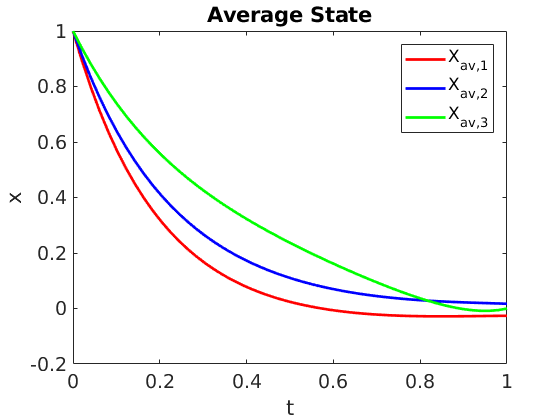
\includegraphics[width=\textwidth]{xav.png}
        \caption{Average state vector components.}
        \label{fig:averageStateVector}
    \end{subfigure}
    ~ %add desired spacing between images, e. g. ~, \quad, \qquad, \hfill etc. 
      %(or a blank line to force the subfigure onto a new line)
    \begin{subfigure}[b]{0.4\textwidth}
        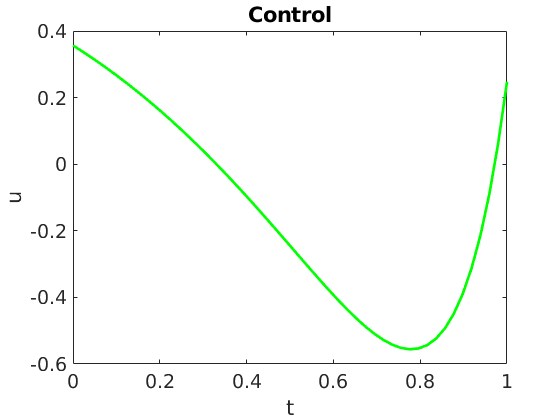
\includegraphics[width=\textwidth]{u.png}
        \caption{Control.}
        \label{fig:Control}
    \end{subfigure}
    ~ %add desired spacing between images, e. g. ~, \quad, \qquad, \hfill etc. 
    %(or a blank line to force the subfigure onto a new line)
    \caption{Control system with $N=3$, $M=1$ and target average state $\bar{x}=[0,0,0]^t$.}\label{fig:Results1}
\end{figure}

\begin{figure}[h]
  \centering
      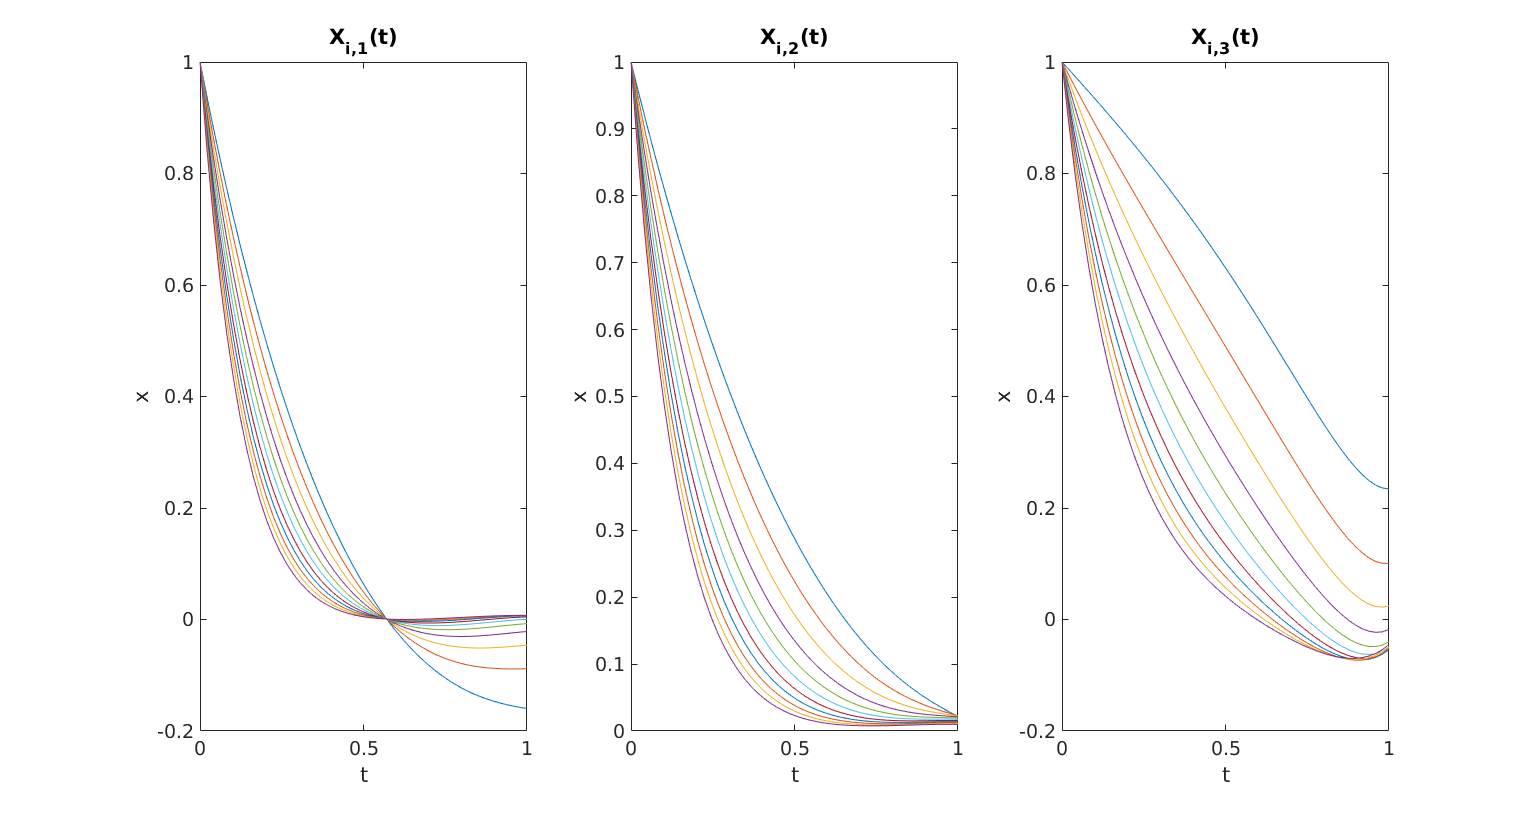
\includegraphics[width=1\textwidth]{xi.png}
  \caption{State vector components for every parameter $\nu_i$. One can observe that the final state $x\left(T, \nu_i \right)$ is not close to $\bar{x}=[0,0,0]^t$ in general.}
\end{figure}

\begin{thebibliography}{1}
\bibitem{averagedcontrolzuazua} 
E. Zuazua (2014). Averaged Control. \textit{Automatica}, 50 (12), p. 3077-3087.
\end{thebibliography}

\end{document}